\section*{Problemas PI:}

Para os problemas apresentados, realizar:
\begin{enumerate}[label=\alph*)]
    \item Simulação usando MATLAB/Simulink realizando análise dos resultados com relação a estabilidade e 
    resposta dinâmica do sistema
    \item Analisar o LGR sem/com controlador
    \item Determine o tempo de amostragem e realize a discretização dos controladores. Comparar com a
    solução continua.
    \item Discretizar os sistemas (controlador e planta) e analisar a estabilidade usando o método de Jury e
    Routh Hurwitz.
\end{enumerate}
    

\subsection*{Problema 1:}

Para esse problema, o modelo de um motor possui como FT a equação \ref{eq:Gp1}. 

\begin{equation}
    G_p = \frac{4}{s^3+3s^2+10s}
    \label{eq:Gp1}
\end{equation}

A FT de MF, com um controlador proporcional é o visto na equação \ref{eq:Gmf1}.

\begin{equation}
    Gmf = \frac{4kp}{s^3+3s^2+10s + 4kp}
    \label{eq:Gmf1}
\end{equation}

Foi visto no desenvolvimento da questão que para o sistema ser estável o ganho propocional deve estar
no intervalo: $0<kp<7,5$. Foi determinado $kp = 4$.


\subsubsection*{a)}
    A estabilidade do sistema foi verificada através de uma entrada ao degrau. Pelo desenvolvimento analítico,
    o erro em regime estacionário deve ser zero a uma entrada ao degrau, espera-se obter o mesmo resultado
    pela simulação no MATLAB através do Código \ref{Q1A}.

    \begin{lstlisting}[language=Matlab,label=Q1A,caption=Análise da estabilidade]
%FT sem controlador
num = 4;
den = [1 3 10 0];
G = tf(num,den);
%FT com controlador
kp = 4;
Gmf = tf(kp*num,[1 3 8 4*kp]);

% a)
[y,t] = step(Gmf);
figure
plot(t, y, 'LineWidth', 2);
legend('c(t)')
grid
    \end{lstlisting}

    A Figura \ref{fig:Q1A} apresenta a resposta do sistema ao degrau.


    \begin{figure}[!h]
        \centering
        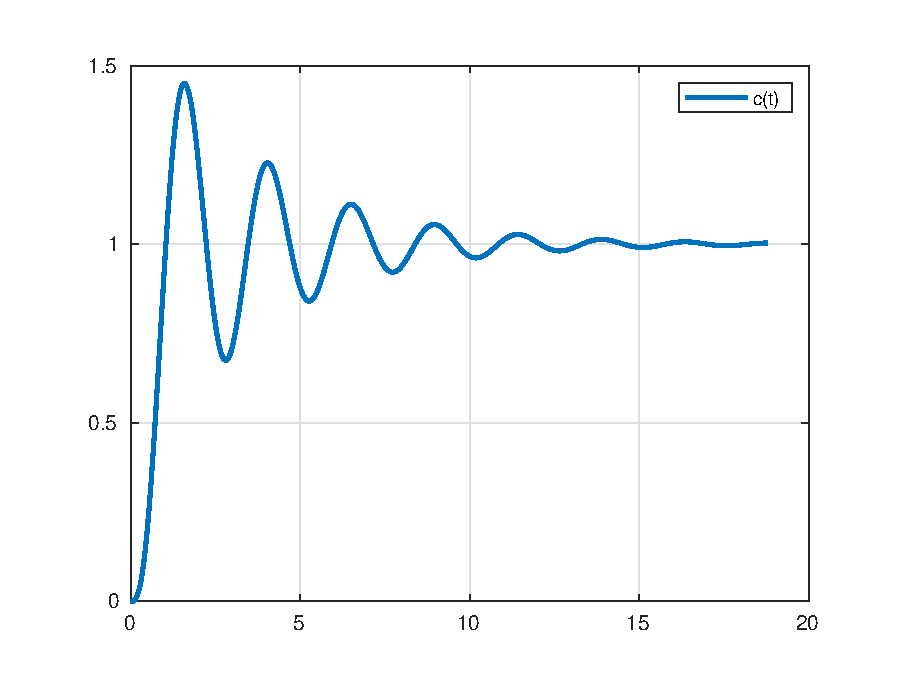
\includegraphics[width = 0.75\linewidth]{Figuras/ProblemasPI/Problema1/step1.eps}
        \caption{Gráfico da resposta ao degrau do sistema}
        \label{fig:Q1A}                   
    \end{figure}

    Podemos verificar que o erro em regime estacionário do sistema tende a zero, assim como determinado 
    através do cálculo analítico.

\subsubsection*{b)}